
\appendix
% the appendix command just changes heading styles for appendices.

\chapter{System and software environment}

\section{ABC SMC implementation}

\subsection{Local machine}

Local development machine is a Mac laptop, running on macOS 10.15.6. The environment of the development is listed in Table \ref{table:local_macine}.

\begin{table}[h!]
    \centering
    \begin{tabular}{|c c|}
        \hline
        Environment                 & Version                       \\ [0.5ex]
        \hline\hline
        $\lambda_N$                 & 2.1989                        \\
        $\kappa_{N\beta}$           & 3.9627                        \\
        $\mu_N$                     & 1.7219                        \\
        $\nu_{N\Phi}$  0.2195       & $cell^{-1}\cdotp h^{-1}$      \\
        \hline
        $\lambda_\Phi$              & 1.3146  $cell/h$              \\
        $\kappa_{\Phi\beta}$ 0.1235 & $cell/(unit\cdotp h)$         \\
        $\mu_\Phi$  0.1454          & $h^{-1}$                      \\
        \hline
        $s_{\beta N}$               & 6.5536  $unit/(cell\cdotp h)$ \\
        $i_{\beta\Phi}$  1.7062     & $cell^{-1}$                   \\
        $\mu_\beta$                 & 0.5212  $h^{-1}$              \\
        \hline
        $s_{\alpha\Phi}$  10.2416   & $unit/(cell\cdotp h)$         \\
        $\mu_\alpha$ 19.6642        & $h^{-1}$                      \\
        [1ex]
        \hline
    \end{tabular}
    \caption{Environment on local machine}
    \label{table:local_macine}
\end{table}

\subsection{Remote machine}

\begin{table}[h!]
    \centering
    \begin{tabular}{|c c|}
        \hline
        Environment                 & Version                       \\ [0.5ex]
        \hline\hline
        $\lambda_N$                 & 2.1989                        \\
        $\kappa_{N\beta}$           & 3.9627                        \\
        $\mu_N$                     & 1.7219                        \\
        $\nu_{N\Phi}$  0.2195       & $cell^{-1}\cdotp h^{-1}$      \\
        \hline
        $\lambda_\Phi$              & 1.3146  $cell/h$              \\
        $\kappa_{\Phi\beta}$ 0.1235 & $cell/(unit\cdotp h)$         \\
        $\mu_\Phi$  0.1454          & $h^{-1}$                      \\
        \hline
        $s_{\beta N}$               & 6.5536  $unit/(cell\cdotp h)$ \\
        $i_{\beta\Phi}$  1.7062     & $cell^{-1}$                   \\
        $\mu_\beta$                 & 0.5212  $h^{-1}$              \\
        \hline
        $s_{\alpha\Phi}$  10.2416   & $unit/(cell\cdotp h)$         \\
        $\mu_\alpha$ 19.6642        & $h^{-1}$                      \\
        [1ex]
        \hline
    \end{tabular}
    \caption{Environment on remote machine}
    \label{table:remote_macine}
\end{table}

\section{Data analysis}

\chapter{Data and settings}






\section{Infer-back experiments}

\subsection{Parameter values used to generate synthetic data}

\begin{table}[h!]
    \centering
    \begin{tabular}{|c c c|}
        \hline
        Parameter            & Value & Unit                     \\ [0.5ex]
        \hline\hline
        $\lambda_N$          & 2.20  & $cell/h$                 \\
        $\kappa_{N\beta}$    & 3.96  & $cell/(unit\cdotp h)$    \\
        $\mu_N$              & 1.72  & $h^{-1}$                 \\
        $\nu_{N\Phi}$        & 0.220 & $cell^{-1}\cdotp h^{-1}$ \\
        \hline
        $\lambda_\Phi$       & 1.31  & $cell/h$                 \\
        $\kappa_{\Phi\beta}$ & 0.124 & $cell/(unit\cdotp h)$    \\
        $\mu_\Phi$           & 0.145 & $h^{-1}$                 \\
        \hline
        $s_{\beta N}$        & 6.554 & $unit/(cell\cdotp h)$    \\
        $i_{\beta\Phi}$      & 1.71  & $cell^{-1}$              \\
        $\mu_\beta$          & 0.521 & $h^{-1}$                 \\
        \hline
        $s_{\alpha\Phi}$     & 10.2  & $unit/(cell\cdotp h)$    \\
        $\mu_\alpha$         & 19.1  & $h^{-1}$                 \\
        \hline
    \end{tabular}
    \caption{Parameter values used for model 1}
    \label{table:m1}
\end{table}

\subsection{Kernel experiment: median epsilon schedule}

\begin{figure}[h!]

    \begin{center}
        \resizebox{1.0\hsize}{!}{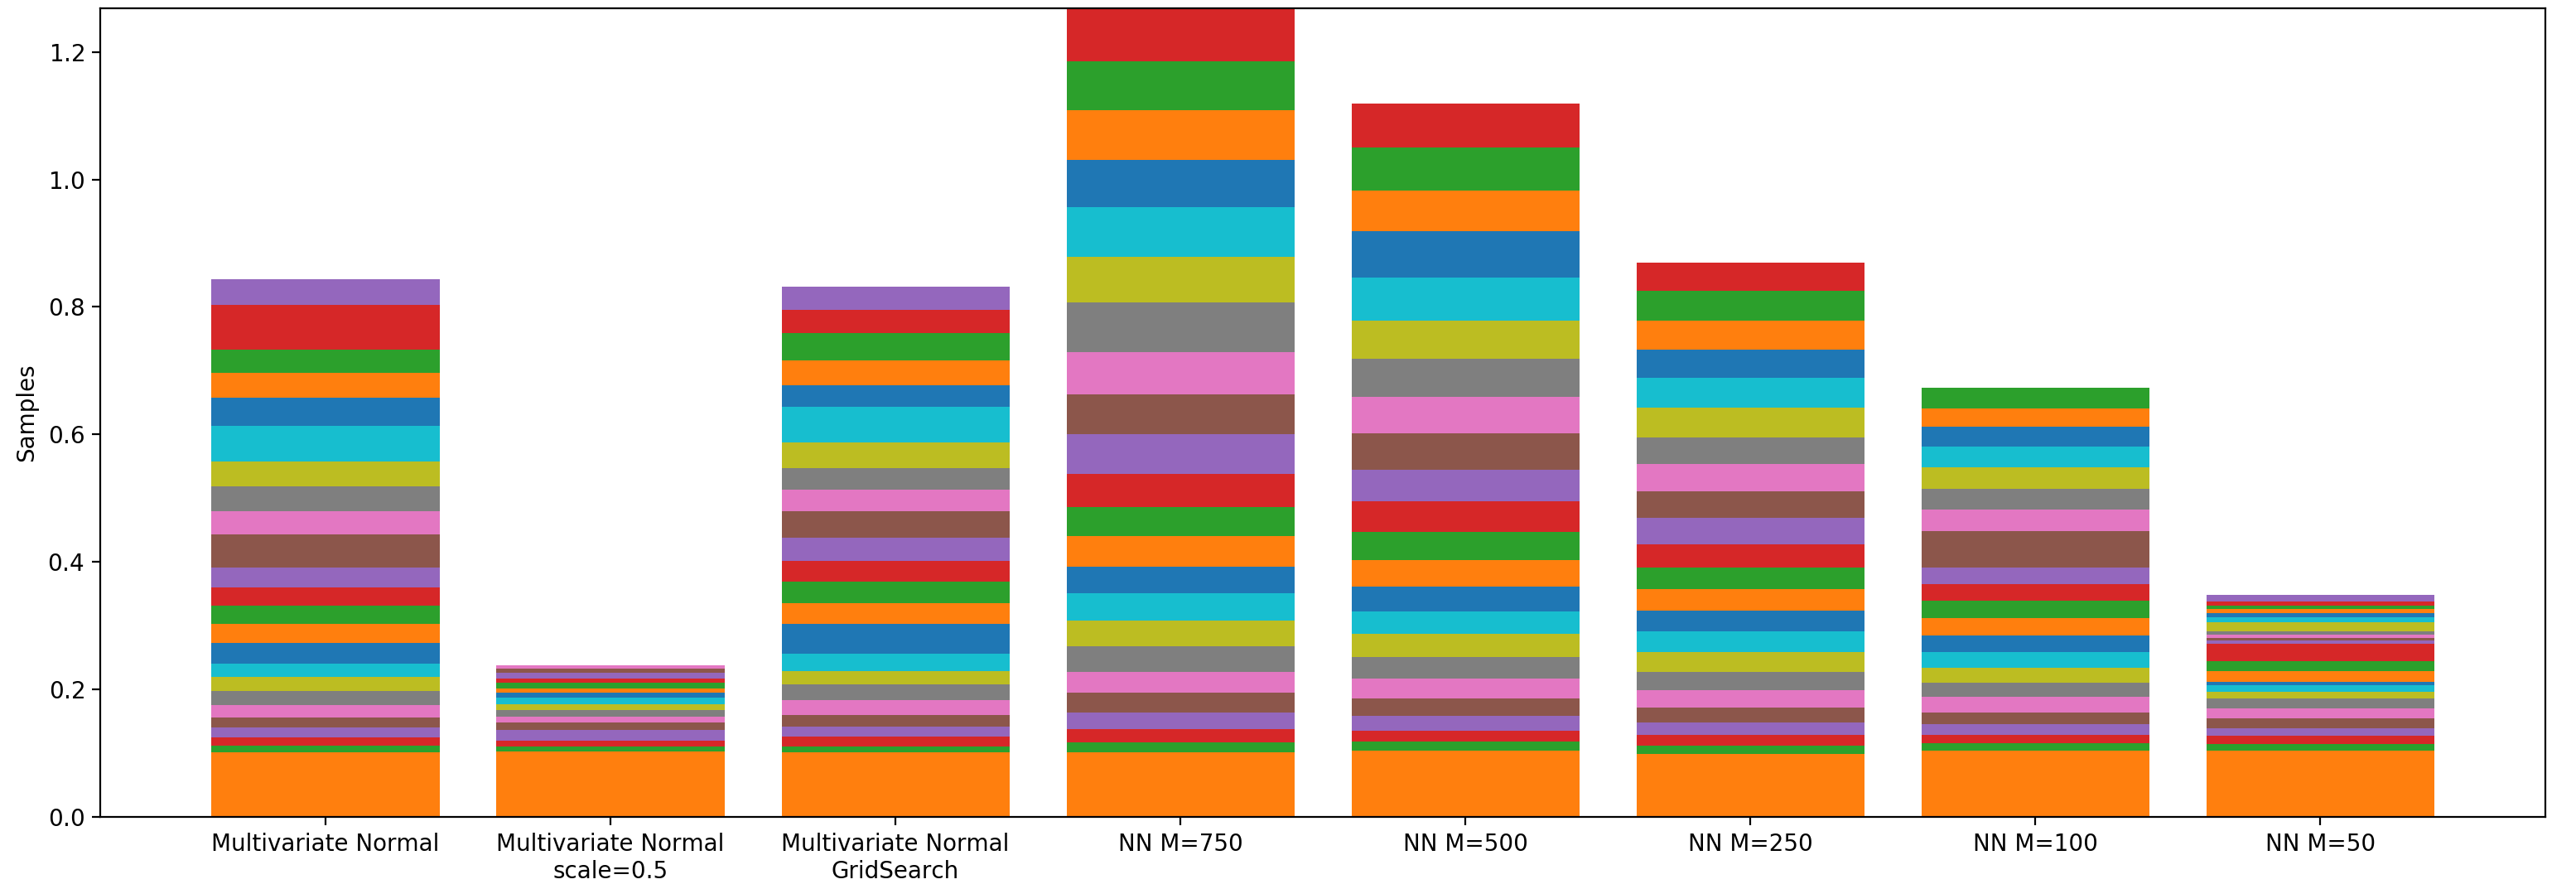
\includegraphics{fig/kernel2.png}}
    \end{center}

    \caption[Total sampling size of different kernels, using median epsilon strategy]
    {Total sampling size of different kernels, using median epsilon strategy. Different color represents different generations (bottom to top: population 1 to population 20)}
    \label{fig:kernel2}

    \begin{center}
        \resizebox{1.0\hsize}{!}{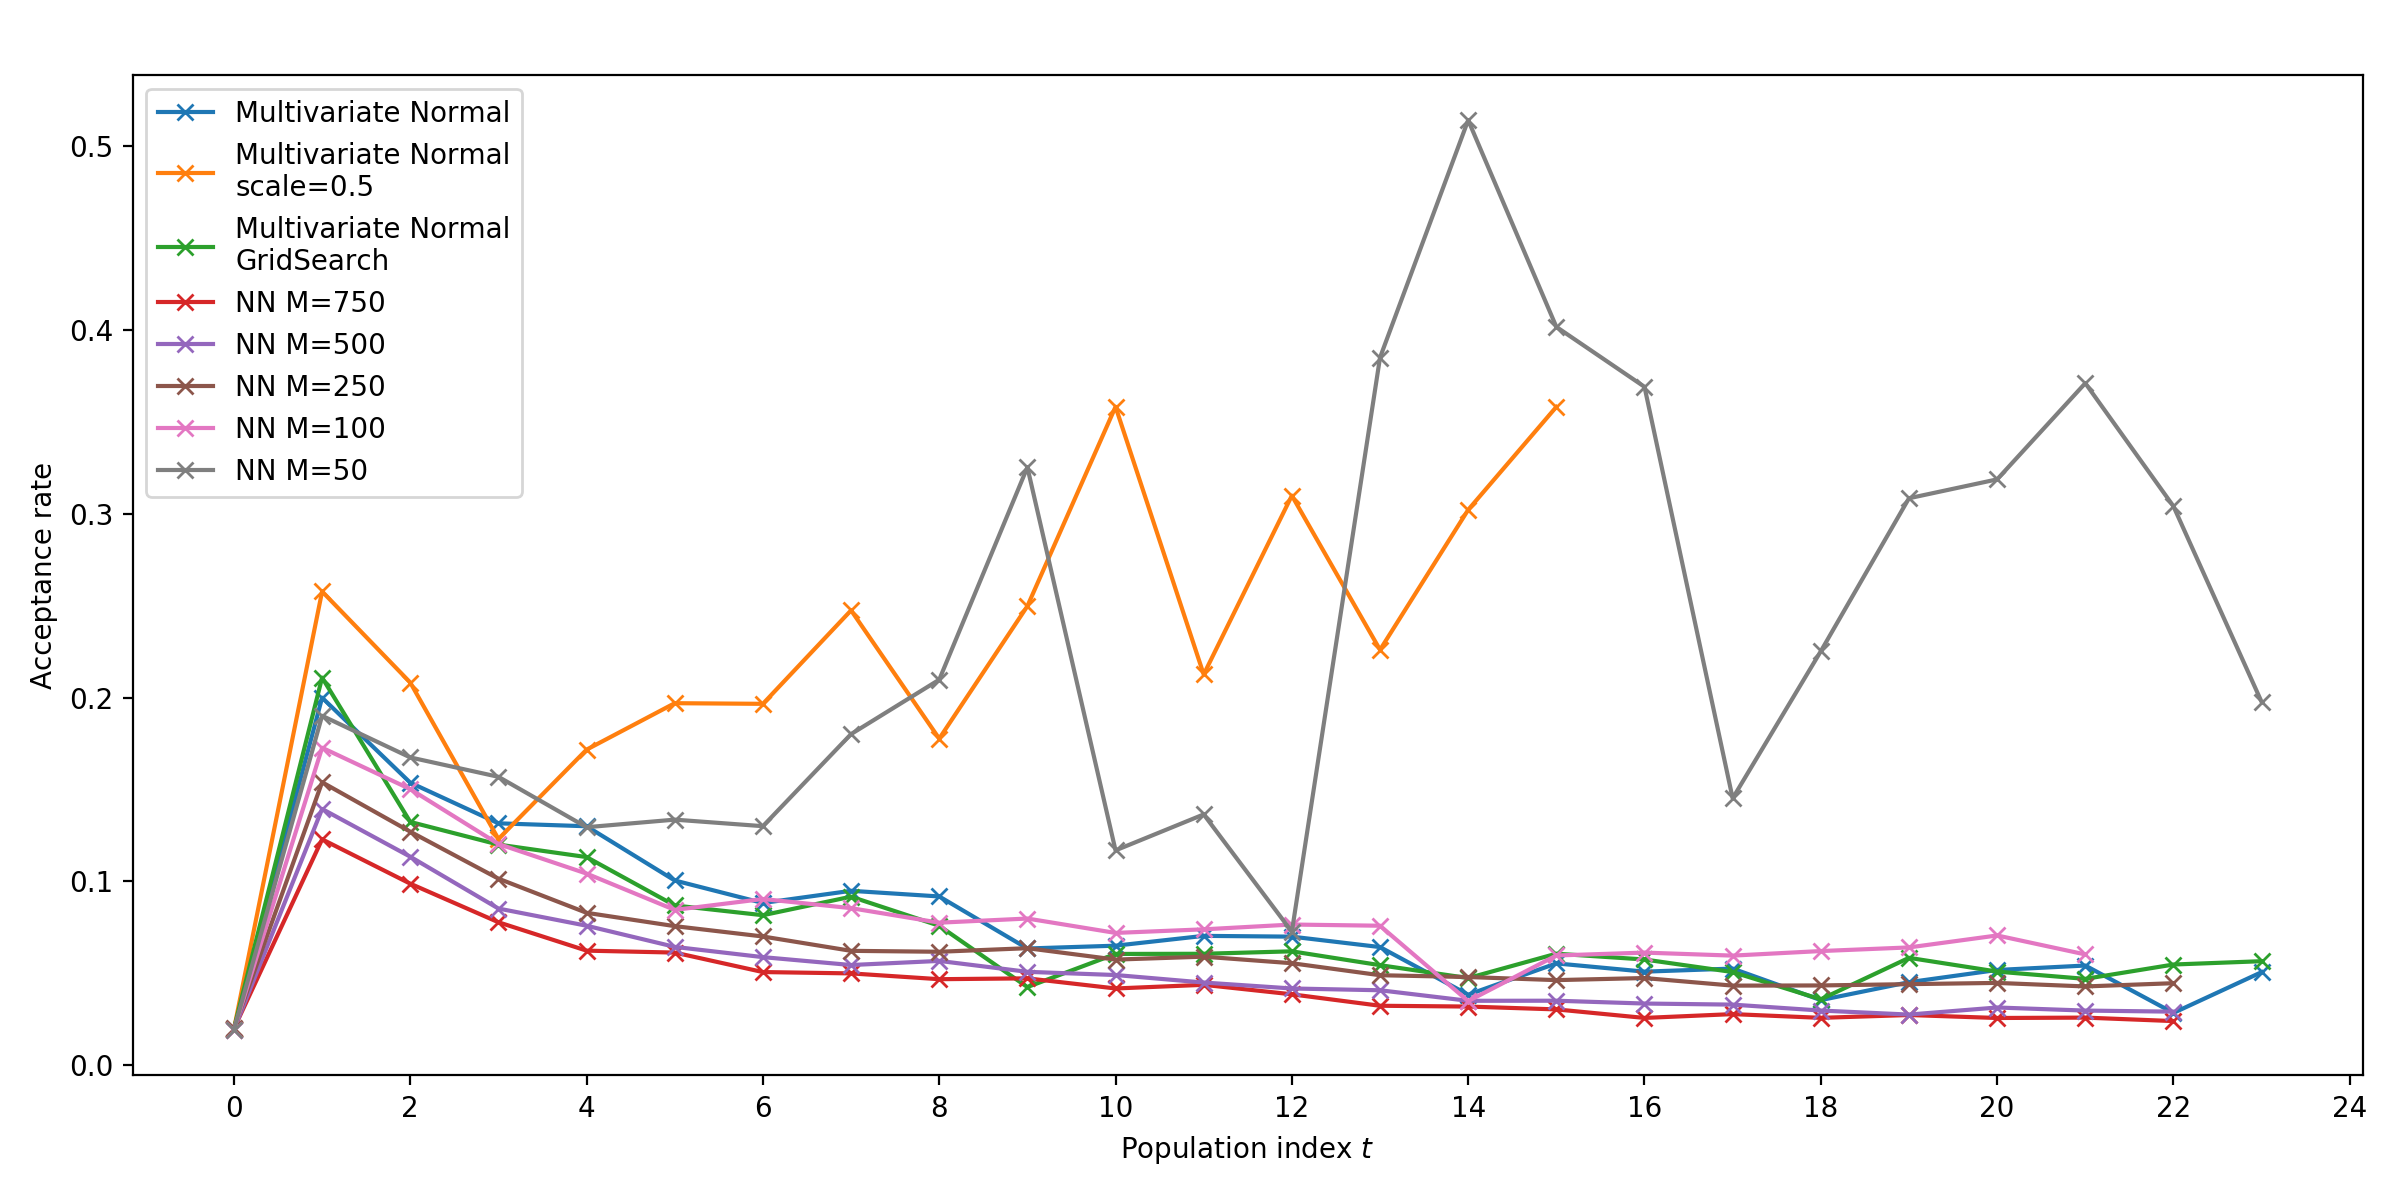
\includegraphics{fig/acceptance2.png}}
    \end{center}

    \caption[Acceptance rates of different kernels, using median epsilon strategy]
    {Acceptance rates of different kernels, using median epsilon strategy. Each population has 2000 particles}
    \label{fig:acceptance2}

\end{figure}


\section{Parameter inference and model comparison results}

\begin{figure}[H]

    \begin{center}
        \resizebox{1.0\hsize}{!}{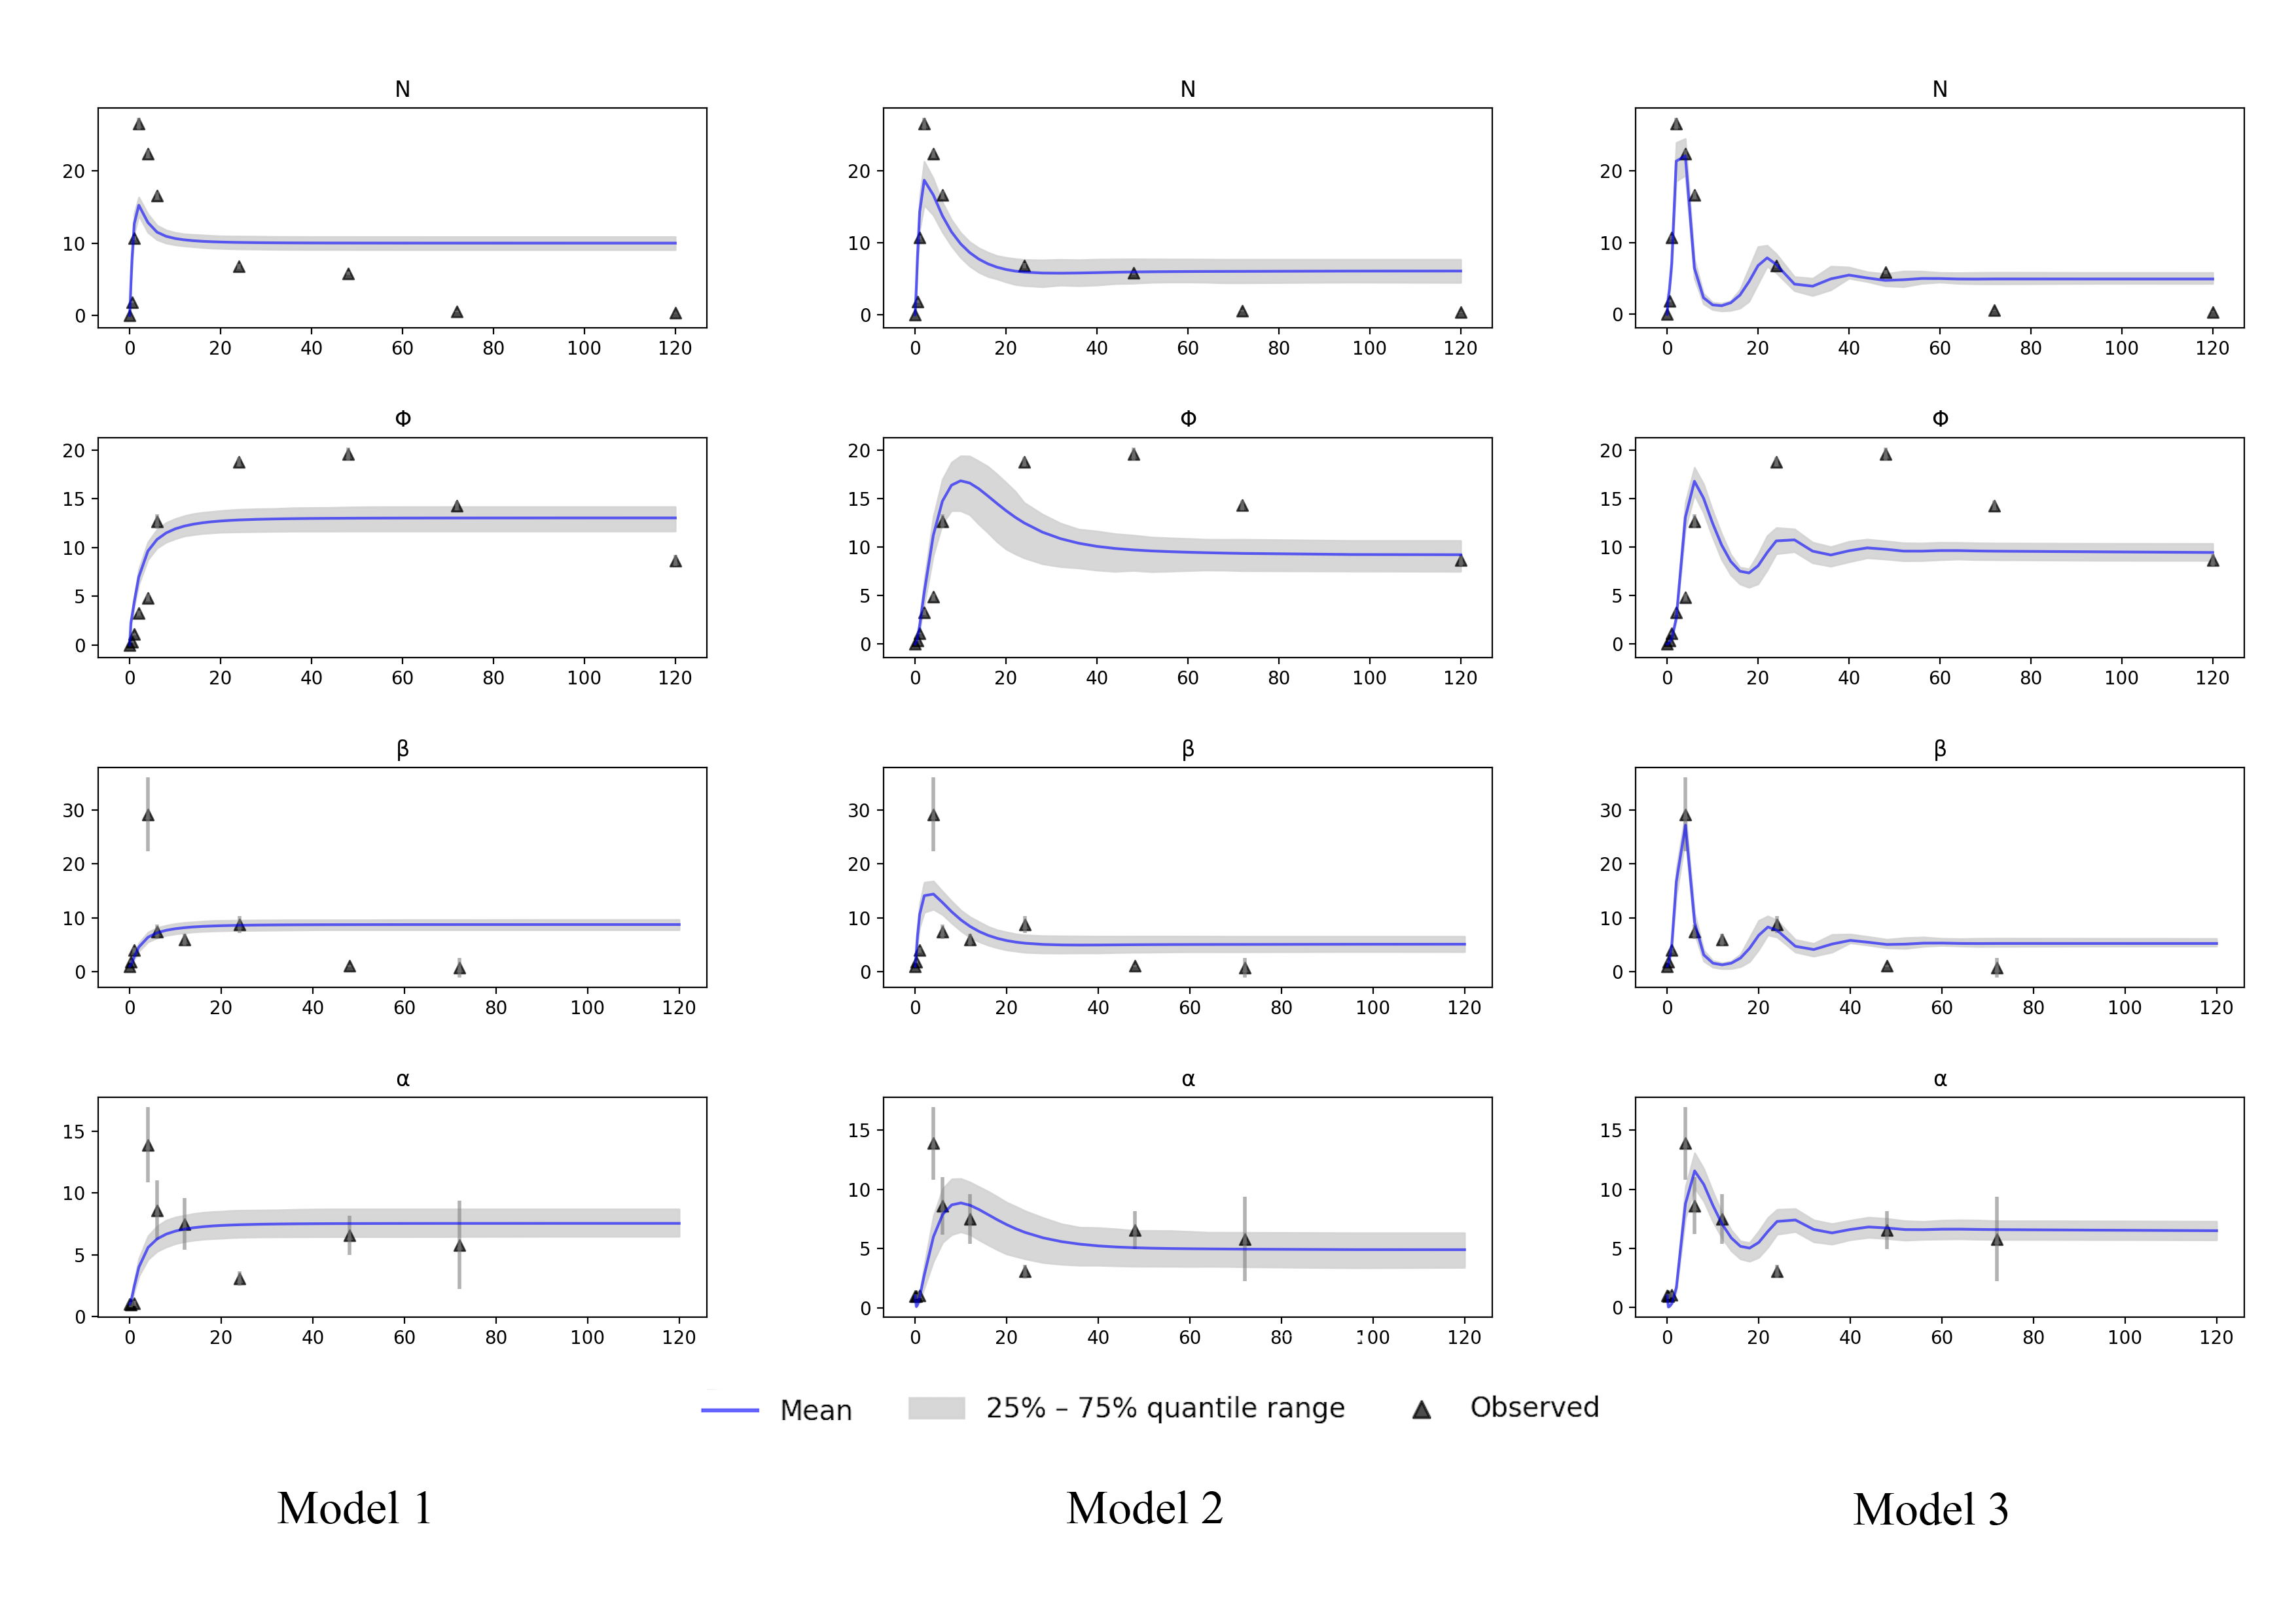
\includegraphics{fig/resultCurve_uni.png}}
    \end{center}

    \caption{Total sampling size}
    \label{fig:resultCurve_uni}


\end{figure}






